\documentclass[compress]{beamer}

\beamertemplatetransparentcovered

\usepackage{hyperref}
\usepackage{textcomp}

\usetheme{Ubuntu}

\graphicspath{{./images/}}

\title{Ubuntu România}
\subtitle{Comunitatea Românească Ubuntu}

\author{Mihai Maruseac (\href{mailto:mihai.maruseac@rosedu.org}{mihai.maruseac@rosedu.org})}
\date{12 Noiembrie, 2012}

\institute{Programatica 2012, București, România}

\begin{document}

% ----------------------------------------------------------------------------
% *** Titlepage <<<
% ----------------------------------------------------------------------------
\maketitle
% ----------------------------------------------------------------------------
% *** END of Titlepage >>>
% ----------------------------------------------------------------------------


% ----------------------------------------------------------------------------
% *** Frame <<<
% ----------------------------------------------------------------------------
\begin{frame}
  \begin{center}
    \large
    „Ubuntu” este un cuvânt vechi african,
    însemnând „umanitate către ceilalți (semenii noștri)”.
    Ubuntu se poate traduce, de asemenea, și prin
    „eu sunt ceea ce sunt datorită a ceea ce suntem noi toți”.
    \\
    Distribuția Ubuntu Linux aduce spiritul Ubuntu în lumea software-ului.
  \end{center}
\end{frame}
% ----------------------------------------------------------------------------
% *** END of Frame >>>
% ----------------------------------------------------------------------------

% ----------------------------------------------------------------------------
% *** Frame <<<
% ----------------------------------------------------------------------------
\begin{frame}
\frametitle{Despre Ubuntu}

\begin{itemize}[<+->]
  \item este un sistem de operare bazat pe Linux
  \item este disponibil gratuit
  \item are suport atât din partea comunității cât și comercial
  \item este reprezentat în toată lumea prin comunități locale, numite și LoCo
  \item este probabil cea mai populară distribuție pentru desktop
  \item a pornit din Debian și este în continuare bazat pe Debian
  \item are versiuni pentru desktop, netbook și server
\end{itemize}
\end{frame}
% ----------------------------------------------------------------------------
% *** END of Frame >>>
% ----------------------------------------------------------------------------

% ----------------------------------------------------------------------------
% *** Frame <<<
% ----------------------------------------------------------------------------
\begin{frame}
\frametitle{Promisiunile Ubuntu}

\small
\begin{itemize}[<+->]
  \item Ubuntu va fi întotdeauna gratuit și nu se percepe nici un fel de taxă pentru ediția enterprise (destinată companiilor), noi facem ca munca noastră de cea mai bună calitate să fie disponibilă tuturor sub aceleași condiții \bf gratuite.
  \item Ubuntu ofera ceea ce este mai bun în software-ul liber, adunând și integrând
  cele mai bune aplicații libere.
  \item Ubuntu include ceea ce este mai bun în infrastructura de traduceri și accesibilitate pe care comunitatea software-ului liber o are de oferit pentru a face Ubuntu utilizabil de cât mai multe persoane posibil.
  \item Noile versiuni Ubuntu sunt lansate cu regularitate; o nouă versiune este realizată de regulă la fiecare șase luni. Puteți folosi versiunea curentă stabilă sau versiunea curentă de dezvoltare. Pentru versiunea curentă se oferă suport tehnic prin actualizări pe o perioadă de cel puțin 18 luni.
  \item Ubuntu este angajat în totalitate principiilor dezvoltării de software gratuit și liber; încurajăm ca oricine să folosească software-ul gratuit și liber, să-l îmbunătățească și să-l distribuie mai departe.
\end{itemize}
\end{frame}
% ----------------------------------------------------------------------------
% *** END of Frame >>>
% ----------------------------------------------------------------------------

% ----------------------------------------------------------------------------
% *** Frame <<<
% ----------------------------------------------------------------------------
\begin{frame}
\frametitle{Ubuntu în lume}

\begin{itemize}[<+->]
  \item și-a început activitatea 2005
  \item în Iunie 2006 a apărut prima versiune cu suport prelungit (LTS) pentru 4 ani
  \item parteneriate cu Dell, Asus, \ldots pentru servere și laptopuri
  \item cel mai folosit sistem de operare în cloud (Amazon AWS)
  \item versiune beta pentru TV-uri
  \item momentan se lucrează și la Ubuntu pe platforme mobile
\end{itemize}

\end{frame}
% ----------------------------------------------------------------------------
% *** END of Frame >>>
% ----------------------------------------------------------------------------

% ----------------------------------------------------------------------------
% *** Frame <<<
% ----------------------------------------------------------------------------
\begin{frame}
\frametitle{Ubuntu în România}

\begin{itemize}[<+->]
  \item și-a început activitatea în comunitatea Linux din Timișoara, $\sim$2005 (TMLUG), în special prin
    \begin{itemize}[<+->]
      \item Dan Damian
      \item Silviu Bojica
      \item Sebastian Ivan
    \end{itemize}
  \item prin 2006-2007 multe activități sunt preluate de către comunitatea Linux din Cluj (CJLUG)
  \item în 2008, coordonarea comunității este preluată de către Adi Roiban
  \item în 2011. coordonarea comunității este preluată de către Alex Cucu
  \item în toți acești ani comunitatea a fost re-aprobată cu success de mai multe ori drept una oficială
\end{itemize}

\end{frame}
% ----------------------------------------------------------------------------
% *** END of Frame >>>
% ----------------------------------------------------------------------------

% ----------------------------------------------------------------------------
% *** Frame <<<
% ----------------------------------------------------------------------------
\begin{frame}
\frametitle{Activitățile echipei ubuntu-ro}

\ldots includ:

\begin{itemize}[<+->]
  \item traducerea și actualizarea traducerilor
  \item întreținerea și administrarea serviciilor online ubuntu.ro și a altor sub-proiecte
  \item distribuirea de CD-uri gratis prin poștă
  \item rapoarte și comunicare cu comunitatea globală
  \item promovare si colaborare cu organizatorii evenimentelor FLOSS
  \item organizarea evenimentelor și întâlnirilor locale
\end{itemize}
\end{frame}
% ----------------------------------------------------------------------------
% *** END of Frame >>>
% ----------------------------------------------------------------------------

% ----------------------------------------------------------------------------
% *** Frame <<<
% ----------------------------------------------------------------------------
\begin{frame}
\frametitle{Despre traduceri}

\begin{itemize}[<+->]
  \item peste 50\% din traduceri sunt acoperite
  \item în principal atenția este orientată spre traducerea interfețelor
  \item \href{https://launchpad.net/~ubuntu-ro/+members}{lista de traducători}
  \item \href{https://translations.launchpad.net/ubuntu/quantal/+lang/ro}{statutul traducerilor la ora actuală}
\end{itemize}
\end{frame}
% ----------------------------------------------------------------------------
% *** END of Frame >>>
% ----------------------------------------------------------------------------

% ----------------------------------------------------------------------------
% *** Frame <<<
% ----------------------------------------------------------------------------
\begin{frame}
\frametitle{Despre servicii online}

\begin{itemize}[<+->]
  \item pe \href{http://ubuntu.ro}{ubuntu.ro} se pot obține majoritatea informațiilor din această prezentare
  \item pe \href{http://forum.ubuntu.ro}{forum.ubuntu.ro} se poate obține ajutorul comunității gratuit

\end{itemize}
\end{frame}
% ----------------------------------------------------------------------------
% *** END of Frame >>>
% ----------------------------------------------------------------------------

% ----------------------------------------------------------------------------
% *** Frame <<<
% ----------------------------------------------------------------------------
\begin{frame}
\frametitle{Despre activități de promovare}

\begin{figure}[ht]
    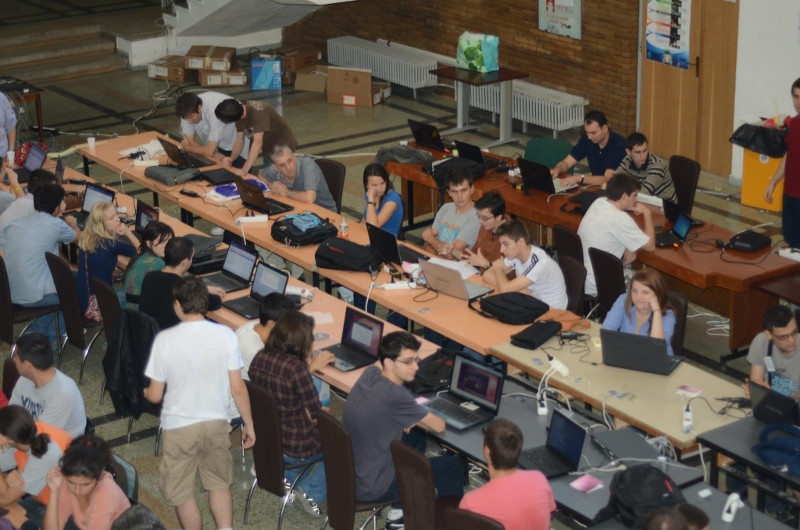
\includegraphics[width=4cm]{./res/lif2012.jpg} % TODO: float righ
\end{figure} 
\begin{itemize}[<+->]
  \item colaborare cu ROSEdu pentru Linux Install Fest
  \item instalare ubuntu pe calculatoare personale, oferind suport tehnic
  \item a 6-a ediție, în Octombrie 2012, a avut peste 100 de participanți
\end{itemize}
\end{frame}
% ----------------------------------------------------------------------------
% *** END of Frame >>>
% ----------------------------------------------------------------------------

% ----------------------------------------------------------------------------
% *** Frame <<<
% ----------------------------------------------------------------------------
\begin{frame}
\frametitle{Cum se poate lua legătura cu noi}

\begin{itemize}[<+->]
  \item prin email la \href{mailto://contact@ubuntu.ro}{contact@ubuntu.ro}
  \item în persoană, la \href{http://camp.softwareliber.ro/}{camp.softwareliber.ro}
\end{itemize}
\end{frame}
% ----------------------------------------------------------------------------
% *** END of Frame >>>
% ----------------------------------------------------------------------------

% ----------------------------------------------------------------------------
% *** Frame <<<
% ----------------------------------------------------------------------------
\begin{frame}
  \begin{center}
    \huge
    Mulțumim pentru atenție!
    \\
    Întrebări\ldots
    \\
    (\href{mailto://contact@ubuntu.ro}{contact@ubuntu.ro})
  \end{center}
\end{frame}
% ----------------------------------------------------------------------------
% *** END of Frame >>>
% ----------------------------------------------------------------------------

\end{document}
